\documentclass[11pt,a4paper]{article}
\usepackage[utf8]{inputenc}
\usepackage[T1]{fontenc}
\usepackage{geometry}
\usepackage{graphicx}
\usepackage{listings}
\usepackage{xcolor}
\usepackage{hyperref}
\usepackage{float}
\usepackage{enumitem}
\usepackage{booktabs}
\usepackage{fancyhdr}
\usepackage{titlesec}
\usepackage{tcolorbox}
\usepackage{parskip}
\usepackage{caption}
\usepackage{tikz}
\usetikzlibrary{shapes.geometric, arrows.meta, positioning, fit, backgrounds}

\geometry{margin=2.5cm}

\hypersetup{
    colorlinks=true,
    linkcolor=blue!70!black,
    urlcolor=blue!60!black,
    citecolor=blue!70!black
}

\definecolor{codebg}{RGB}{245,245,245}
\definecolor{codeframe}{RGB}{200,200,200}
\definecolor{codegreen}{RGB}{40,160,40}
\definecolor{codepurple}{RGB}{130,80,180}
\definecolor{codegray}{RGB}{100,100,100}
\definecolor{tealaccent}{RGB}{15,118,110}

\lstdefinestyle{codestyle}{
    backgroundcolor=\color{codebg},
    frame=single,
    rulecolor=\color{codeframe},
    basicstyle=\ttfamily\small,
    breaklines=true,
    columns=fullflexible,
    keepspaces=true,
    showstringspaces=false,
    xleftmargin=0.5cm,
    xrightmargin=0.5cm,
    aboveskip=0.5em,
    belowskip=0.5em,
    keywordstyle=\color{codepurple}\bfseries,
    stringstyle=\color{codegreen},
    commentstyle=\color{codegray}\itshape,
}

\newtcolorbox{rationale}{
    colback=blue!5!white, colframe=blue!40!black,
    title=Design Rationale, fonttitle=\bfseries,
    boxrule=0.5pt, arc=2mm,
}
\newtcolorbox{designnote}{
    colback=yellow!8!white, colframe=orange!60!black,
    title=Key Insight, fonttitle=\bfseries,
    boxrule=0.5pt, arc=2mm,
}
\newtcolorbox{successbox}[1]{
    colback=green!5!white, colframe=green!40!black,
    title=#1, fonttitle=\bfseries,
    boxrule=0.5pt, arc=2mm,
}
\newtcolorbox{reflectionbox}{
    colback=purple!5!white, colframe=purple!40!black,
    title=Reflection, fonttitle=\bfseries,
    boxrule=0.5pt, arc=2mm,
}

\pagestyle{fancy}
\fancyhf{}
\fancyhead[L]{\small Seismic Command --- MCP Integration}
\fancyhead[R]{\small Yunus Emre Balci}
\fancyfoot[C]{\thepage}

\title{\textbf{Model Context Protocol Integration in\\Seismic Command: Architecture, Implementation, and Live Demo}}
\author{Yunus Emre Balci \\ Akdeniz University --- Computer Engineering}
\date{May 2026 \\[0.3em]\small
Stack: FastMCP (Python) \textbullet{} Angular 18 \textbullet{} LangGraph \textbullet{} Spring Boot}

\begin{document}

\maketitle
\thispagestyle{fancy}
\tableofcontents
\newpage

% ============================================================
\section{Introduction}
% ============================================================

Seismic Command is a full-stack earthquake intelligence platform that combines a
Spring Boot data backend, a Python LangGraph orchestration service, and an Angular
frontend. This report documents the integration of the \textbf{Model Context
Protocol (MCP)} into Seismic Command and explains why MCP was chosen, how it was
implemented, and how the protocol works end-to-end.

\begin{rationale}
MCP (Model Context Protocol) is an open protocol developed by Anthropic that gives
AI models a \textit{standardised interface} to tools, resources, and data sources.
Without MCP, every consumer of the earthquake data (the chat agent, the risk
assessment, a future mobile app, an external AI assistant) would need its own
bespoke integration. With MCP, a single server exposes all capabilities and any
compliant host can discover and invoke them automatically.

Concretely, Seismic Command benefits from MCP in three ways:
\begin{itemize}[leftmargin=1.2em]
    \item \textbf{Standardisation:} tool schemas are discovered at runtime via
          \texttt{tools/list}; no hard-coded API surface in every consumer.
    \item \textbf{Reuse:} the LangGraph chat agent and the live demo page both
          talk to \emph{the same} MCP endpoint.
    \item \textbf{Openness:} Claude Desktop, Cursor, or any MCP-capable host can
          be pointed at \texttt{http://localhost:8002/mcp/} and gain instant
          access to all earthquake tools without additional code.
\end{itemize}
\end{rationale}

\noindent\textbf{Source code:} \url{https://github.com/YunusEmre3757/advenced_web.git}

% ============================================================
\section{System Architecture}
% ============================================================

\subsection{High-Level Overview}

The system has four tiers. Figure~\ref{fig:arch} shows how they relate.

\begin{figure}[H]
\centering
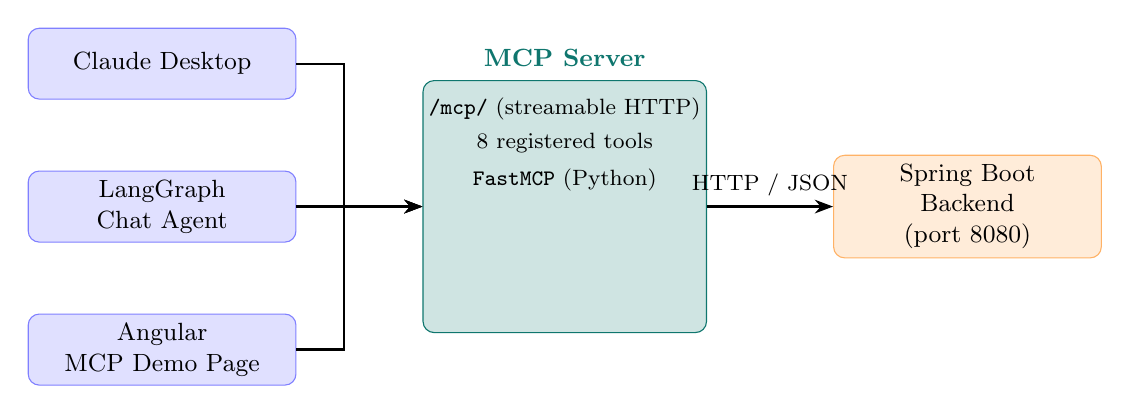
\begin{tikzpicture}[
    node distance=0.9cm and 1.6cm,
    box/.style={rectangle, rounded corners=4pt, minimum width=3.4cm,
                minimum height=0.9cm, align=center, font=\small},
    arr/.style={-Stealth, thick},
]

% Column 1 — Consumers
\node[box, fill=blue!12, draw=blue!50]   (cd)  {Claude Desktop};
\node[box, fill=blue!12, draw=blue!50, below=of cd]  (ag)  {LangGraph\\Chat Agent};
\node[box, fill=blue!12, draw=blue!50, below=of ag]  (ui)  {Angular\\MCP Demo Page};

% Column 2 — MCP Layer
\node[box, fill=tealaccent!20, draw=tealaccent, right=of ag, yshift=0cm,
      minimum height=3.2cm, minimum width=3.6cm] (mcp) {};
\node[font=\small\bfseries, text=tealaccent, above=0.05cm of mcp.north]
      {MCP Server};
\node[font=\footnotesize, below=0.1cm of mcp.north]
      {\texttt{/mcp/} (streamable HTTP)};
\node[font=\footnotesize, below=0.55cm of mcp.north]
      {8 registered tools};
\node[font=\footnotesize, below=1.0cm of mcp.north]
      {\texttt{FastMCP} (Python)};

% Column 3 — Spring
\node[box, fill=orange!15, draw=orange!60, right=of mcp]
      (spring) {Spring Boot\\Backend\\(port 8080)};

% Arrows consumers → MCP
\draw[arr] (cd.east) -- ++(0.6,0) |- (mcp.west);
\draw[arr] (ag.east) -- (mcp.west);
\draw[arr] (ui.east) -- ++(0.6,0) |- (mcp.west);

% Arrow MCP → Spring
\draw[arr] (mcp.east) -- node[above,font=\footnotesize]{HTTP / JSON} (spring.west);

\end{tikzpicture}
\caption{High-level MCP architecture. Three consumers share one MCP server.}
\label{fig:arch}
\end{figure}

\subsection{Protocol Stack}

The MCP server runs inside the same Python process as the LangGraph service.
Table~\ref{tab:stack} lists every component involved.

\begin{table}[H]
\centering
\begin{tabular}{@{}lll@{}}
\toprule
\textbf{Layer} & \textbf{Component} & \textbf{Technology} \\
\midrule
Data             & Spring Boot backend  & Java, REST/JSON \\
MCP Server       & \texttt{seismic\_server.py}   & FastMCP, Python \\
MCP Client       & \texttt{seismic\_client.py}   & mcp-python SDK, streamable HTTP \\
Orchestration    & LangGraph chat graph & Python, LangChain \\
API Gateway      & \texttt{api.py}               & FastAPI, Uvicorn \\
Frontend         & Angular 18 SPA       & TypeScript, Signals \\
\bottomrule
\end{tabular}
\caption{Technology stack for the MCP integration.}
\label{tab:stack}
\end{table}

% ============================================================
\section{MCP Server Implementation}
% ============================================================

\subsection{Server Initialisation}

The server is created with \texttt{FastMCP} and mounted onto the FastAPI application
so that it is reachable at \texttt{/mcp/}:

\begin{lstlisting}[style=codestyle, language=Python]
# seismic_server.py
from mcp.server.fastmcp import FastMCP

mcp = FastMCP(
    "seismic-command-mcp",
    instructions="Provides earthquake-domain tools for Seismic Command.",
    streamable_http_path="/",
)
\end{lstlisting}

\begin{lstlisting}[style=codestyle, language=Python]
# api.py — mount + lifespan
seismic_mcp_app = seismic_mcp.streamable_http_app()

@asynccontextmanager
async def lifespan(_app):
    async with seismic_mcp.session_manager.run():  # MCP alive
        yield
    ...

app.mount("/mcp", seismic_mcp_app)   # reachable at /mcp/
\end{lstlisting}

\begin{designnote}
Mounting the MCP server \emph{inside} the FastAPI app means no separate process is
required. Claude Desktop, Cursor, or any other MCP host simply adds
\texttt{http://localhost:8002/mcp/} as an HTTP MCP server and instantly has access
to all eight tools without any extra configuration.
\end{designnote}

\subsection{Registered Tools}

Table~\ref{tab:tools} documents all eight tools exposed by the server.

\begin{table}[H]
\centering
\begin{tabular}{@{}p{4.8cm}p{4.4cm}p{4.8cm}@{}}
\toprule
\textbf{Tool} & \textbf{Key parameters} & \textbf{Spring endpoints used} \\
\midrule
\texttt{get\_recent\_earthquakes}   & hours, min\_magnitude, limit           & \texttt{/api/earthquakes/recent} \\
\texttt{get\_seismic\_context}      & latitude, longitude, radius\_km        & recent + historical + fault-lines (parallel) \\
\texttt{get\_earthquake\_detail}    & event\_id                              & \texttt{/api/earthquakes/\{id\}} + aftershocks + similar + dyfi + shakemap \\
\texttt{get\_historical\_events}    & years, min\_magnitude                  & \texttt{/api/historical/events} \\
\texttt{get\_seismic\_gaps}         & ---                                    & \texttt{/api/historical/gaps} \\
\texttt{get\_fault\_lines}          & bbox (min/max lon/lat)                 & \texttt{/api/fault-lines} \\
\texttt{geocode\_address}           & query                                  & \texttt{/api/geocode/search} \\
\texttt{assess\_building\_risk}     & lat, lon, year, floors, soil, system   & recent + historical + fault-lines (parallel) \\
\bottomrule
\end{tabular}
\caption{MCP tools registered on the server.}
\label{tab:tools}
\end{table}

\subsection{Example Tool: \texttt{assess\_building\_risk}}

This tool demonstrates the power of composing multiple data sources inside a single
MCP call. It uses the same \texttt{get\_seismic\_context} tool internally for the
seismic data, then applies a deterministic rule engine to produce a 0--100 risk
score:

\begin{lstlisting}[style=codestyle, language=Python]
@mcp.tool()
async def assess_building_risk(
    latitude: float, longitude: float,
    construction_year: int, floor_count: int,
    soil_type: str = "ZC", structural_system: str = "RC",
    visible_damage: bool = False, radius_km: float = 100.0,
) -> dict[str, Any]:
    """Deterministic structural + seismic risk score (no LLM)."""
    context = await get_seismic_context(
        latitude=latitude, longitude=longitude, radius_km=radius_km
    )
    score = 0
    if construction_year < 1975: score += 35
    elif construction_year < 2000: score += 28
    elif construction_year < 2018: score += 14
    soil_risk = {"ZD": 14, "ZE": 20, "ZF": 25}.get(soil_type, 8)
    score += soil_risk
    if visible_damage: score += 20
    ...
    return {"score": min(score, 100), "level": level, ...}
\end{lstlisting}

% ============================================================
\section{MCP Client Implementation}
% ============================================================

\subsection{Streamable HTTP Transport}

The client in \texttt{seismic\_client.py} communicates with the MCP server over
\textbf{streamable HTTP} using the official \texttt{mcp-python} SDK. This transport
runs JSON-RPC 2.0 messages over a persistent HTTP connection:

\begin{lstlisting}[style=codestyle, language=Python]
from mcp.client.streamable_http import streamable_http_client

class _mcp_session:
    async def __aenter__(self) -> ClientSession:
        self._http_client = httpx.AsyncClient(
            timeout=httpx.Timeout(12.0, read=60.0)
        )
        self._transport = streamable_http_client(
            MCP_SERVER_URL, http_client=self._http_client
        )
        read, write, _ = await self._transport.__aenter__()
        self._session = ClientSession(read, write)
        return await self._session.__aenter__()
\end{lstlisting}

\subsection{Graph Workflow Integration: \texttt{call\_mcp\_tool}}

Any LangGraph node calls earthquake data through MCP via:

\begin{lstlisting}[style=codestyle, language=Python]
async def call_mcp_tool(name: str, arguments: dict) -> dict:
    async with _mcp_session() as session:
        await session.initialize()
        result = await session.call_tool(name, arguments)
    return {
        "tool": name,
        "result": _extract_tool_payload(result),
        "error": None,
    }
\end{lstlisting}

The \texttt{initialize()} call performs the MCP handshake and negotiates the
protocol version before any tool is invoked.

\subsection{Demo Walkthrough: \texttt{run\_mcp\_demo}}

For the live demo page, \texttt{run\_mcp\_demo} performs all protocol steps and
returns them as a structured log that the Angular UI renders step-by-step:

\begin{lstlisting}[style=codestyle, language=Python]
async def run_mcp_demo(tool_name, arguments) -> dict:
    async with _mcp_session() as session:
        init   = await session.initialize()     # step 1
        listed = await session.list_tools()     # step 2
        result = await session.call_tool(       # step 3
                     tool_name, arguments)

    return {
        "transport": "streamable-http",
        "server":    { "name": init.serverInfo.name, ... },
        "steps":     [ connect, initialize, list_tools,
                       call_tool, structured_result ],
        "tools":     [_tool_to_dict(t) for t in listed.tools],
        "result":    _extract_tool_payload(result),
        "explanation": [...],
    }
\end{lstlisting}

% ============================================================
\section{LangGraph Integration}
% ============================================================

\subsection{Hybrid Classifier and Tool Routing}

The chat graph classifies each user question using a keyword fast-path followed by
an LLM structured-output fallback, then routes to the corresponding MCP tool.
Figure~\ref{fig:chatgraph} illustrates the topology.

\begin{figure}[H]
\centering
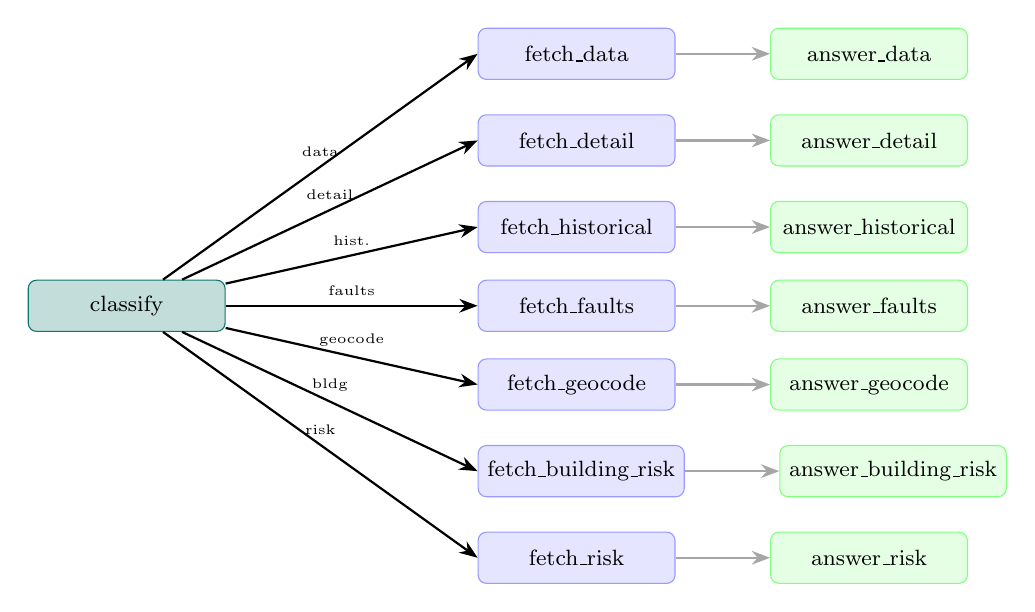
\begin{tikzpicture}[
    node distance=0.55cm and 1.5cm,
    box/.style={rectangle, rounded corners=3pt, minimum width=2.5cm,
                minimum height=0.65cm, align=center, font=\footnotesize},
    arr/.style={-Stealth, thick, gray!70},
    warr/.style={-Stealth, thick},
]
\node[box, fill=tealaccent!25, draw=tealaccent] (cls) {classify};

\node[box, fill=blue!10, draw=blue!40, right=3.2cm of cls, yshift= 3.2cm] (fd) {fetch\_data};
\node[box, fill=blue!10, draw=blue!40, right=3.2cm of cls, yshift= 2.1cm] (fdt) {fetch\_detail};
\node[box, fill=blue!10, draw=blue!40, right=3.2cm of cls, yshift= 1.0cm] (fh) {fetch\_historical};
\node[box, fill=blue!10, draw=blue!40, right=3.2cm of cls, yshift= 0.0cm] (ff) {fetch\_faults};
\node[box, fill=blue!10, draw=blue!40, right=3.2cm of cls, yshift=-1.0cm] (fg) {fetch\_geocode};
\node[box, fill=blue!10, draw=blue!40, right=3.2cm of cls, yshift=-2.1cm] (fb) {fetch\_building\_risk};
\node[box, fill=blue!10, draw=blue!40, right=3.2cm of cls, yshift=-3.2cm] (fr) {fetch\_risk};

\node[box, fill=green!10, draw=green!50, right=1.2cm of fd]  (ad) {answer\_data};
\node[box, fill=green!10, draw=green!50, right=1.2cm of fdt] (adt){answer\_detail};
\node[box, fill=green!10, draw=green!50, right=1.2cm of fh]  (ah) {answer\_historical};
\node[box, fill=green!10, draw=green!50, right=1.2cm of ff]  (af) {answer\_faults};
\node[box, fill=green!10, draw=green!50, right=1.2cm of fg]  (ag2){answer\_geocode};
\node[box, fill=green!10, draw=green!50, right=1.2cm of fb]  (ab) {answer\_building\_risk};
\node[box, fill=green!10, draw=green!50, right=1.2cm of fr]  (ar) {answer\_risk};

\draw[warr] (cls) -- node[above,font=\tiny]{data}    (fd.west);
\draw[warr] (cls) -- node[above,font=\tiny]{detail}  (fdt.west);
\draw[warr] (cls) -- node[above,font=\tiny]{hist.}   (fh.west);
\draw[warr] (cls) -- node[above,font=\tiny]{faults}  (ff.west);
\draw[warr] (cls) -- node[above,font=\tiny]{geocode} (fg.west);
\draw[warr] (cls) -- node[above,font=\tiny]{bldg}    (fb.west);
\draw[warr] (cls) -- node[above,font=\tiny]{risk}    (fr.west);

\draw[arr] (fd) -- (ad);
\draw[arr] (fdt)-- (adt);
\draw[arr] (fh) -- (ah);
\draw[arr] (ff) -- (af);
\draw[arr] (fg) -- (ag2);
\draw[arr] (fb) -- (ab);
\draw[arr] (fr) -- (ar);

\end{tikzpicture}
\caption{Chat graph topology. Each category routes to the appropriate MCP fetch
         node, then to an LLM answer node.}
\label{fig:chatgraph}
\end{figure}

\subsection{Category-to-Tool Mapping}

\begin{table}[H]
\centering
\begin{tabular}{@{}lll@{}}
\toprule
\textbf{Category} & \textbf{MCP Tool} & \textbf{Example trigger} \\
\midrule
\texttt{data}          & \texttt{get\_recent\_earthquakes}  & ``Bu hafta hangi depremler oldu?'' \\
\texttt{detail}        & \texttt{get\_earthquake\_detail}   & ``us7000m9g4 depremi hakkında bilgi'' \\
\texttt{historical}    & \texttt{get\_historical\_events}   & ``Tarihsel büyük depremler'' \\
\texttt{gaps}          & \texttt{get\_seismic\_gaps}        & ``Sismik boşluk analizi'' \\
\texttt{faults}        & \texttt{get\_fault\_lines}         & ``Aktif fay hatları nerede?'' \\
\texttt{geocode}       & \texttt{geocode\_address}          & ``İzmir Konak koordinatı'' \\
\texttt{building\_risk}& \texttt{assess\_building\_risk}    & ``Binam depreme dayanıklı mı?'' \\
\texttt{risk}          & \texttt{get\_seismic\_context}     & ``Bölgem için risk nedir?'' \\
\texttt{guide}         & --- (LLM only)                     & ``Deprem çantasında ne olmalı?'' \\
\texttt{smalltalk}     & --- (LLM only)                     & ``Merhaba'' \\
\bottomrule
\end{tabular}
\caption{Classifier categories and their MCP tool assignments.}
\end{table}

\subsection{Error Handling}

Every fetch node in the graph checks the \texttt{error} field returned by
\texttt{call\_mcp\_tool}. If the MCP server is unreachable, the answer node
immediately returns a user-friendly Turkish message instead of raising an exception:

\begin{lstlisting}[style=codestyle, language=Python]
def _mcp_error_response(mcp_call: dict) -> str | None:
    error = mcp_call.get("error")
    if not error:
        return None
    return (
        "Uzgunum, su anda veri servisine ulasilamiyor. "
        "Lutfen birkac dakika sonra tekrar deneyin. "
        f"(Teknik detay: {error})"
    )
\end{lstlisting}

% ============================================================
\section{Live Demo Page}
% ============================================================

\subsection{Architecture}

The MCP Demo page (\texttt{/mcp-demo}) in the Angular frontend allows any of the
five representative tools to be selected, parameterised, and invoked in real time.
The request passes through:

\[
\text{Angular} \xrightarrow{\text{POST /api/graph/mcp-demo}} \text{Spring proxy}
\xrightarrow{\text{forward}} \text{FastAPI /graph/mcp-demo}
\xrightarrow{\texttt{run\_mcp\_demo()}} \text{MCP /mcp/}
\]

\subsection{Demonstration Tools}

Five tools were selected for the demo page because they each show a distinct
capability and produce results that are immediately readable:

\begin{table}[H]
\centering
\begin{tabular}{@{}lll@{}}
\toprule
\textbf{Demo Tool} & \textbf{Parameters} & \textbf{What it shows} \\
\midrule
Son Depremler          & hours, min\_magnitude, limit        & Real-time data retrieval \\
Sismik Bagflam         & latitude, longitude, radius\_km     & Multi-source parallel fetch \\
Deprem Detayi          & event\_id                           & Event enrichment pipeline \\
Tarihsel Olaylar       & years, min\_magnitude               & Historical archive query \\
Bina Risk Degerlendirmesi & lat, lon, year, floors, soil\ldots & Composite scoring \\
\bottomrule
\end{tabular}
\caption{Tools exposed on the MCP Demo page.}
\end{table}

\subsection{Protocol Steps Rendered in the UI}

For every demo run, the Angular page renders the five protocol steps returned by
\texttt{run\_mcp\_demo}:

\begin{enumerate}[leftmargin=1.5em]
    \item \textbf{MCP HTTP bagflantisi kuruldu} --- client connects to
          \texttt{http://localhost:8002/mcp/}
    \item \textbf{MCP initialize} --- protocol version negotiated,
          server name and capabilities exchanged
    \item \textbf{tools/list} --- all 8 tool schemas discovered at runtime
    \item \textbf{tools/call \textit{<tool\_name>}} --- selected tool invoked
          with typed arguments
    \item \textbf{Yapilandirilmis sonuc} --- JSON result returned to Angular
\end{enumerate}

This step-by-step rendering makes the protocol transparent and directly demonstrates
the \textit{discover then invoke} pattern that is central to MCP.

% ============================================================
\section{Design Decisions}
% ============================================================

\subsection{Streamable HTTP vs.\ stdio Transport}

MCP supports two transports: \textbf{stdio} (subprocess) and
\textbf{streamable HTTP} (persistent HTTP connection). The initial design used
stdio, but streamable HTTP was chosen for the following reasons:

\begin{rationale}
\begin{itemize}[leftmargin=1.2em]
    \item \textbf{No subprocess overhead:} The server is mounted directly into
          FastAPI; no extra process is spawned per request.
    \item \textbf{External accessibility:} Any external MCP host (Claude Desktop,
          Cursor) can connect over HTTP without needing local filesystem access.
    \item \textbf{Lifecycle management:} FastMCP's \texttt{session\_manager} handles
          connection pooling and cleanup inside the FastAPI lifespan context.
\end{itemize}
\end{rationale}

\subsection{Single MCP Server for Multiple Consumers}

Rather than writing bespoke data-fetching code in the chat graph, the building-risk
graph, and the demo page separately, all three consumers call the same MCP server.
This means:

\begin{itemize}[leftmargin=1.2em]
    \item Tool logic is implemented \textit{once} and tested \textit{once}.
    \item Changing a Spring endpoint URL requires updating only
          \texttt{seismic\_server.py}, not every graph.
    \item Adding a new tool automatically makes it available to the chat agent on
          the next deploy, without touching the graph code.
\end{itemize}

\subsection{Deterministic Tool vs.\ LLM Node}

\texttt{assess\_building\_risk} returns a deterministic score (rule engine, no LLM).
The \texttt{/graph/building-risk} endpoint, by contrast, runs the full LangGraph
agentic loop with LLM narrative generation and an evaluator feedback loop. The two
coexist because:

\begin{designnote}
The MCP tool is fast (no LLM tokens consumed), consistent (same inputs always
produce the same score), and suitable for the chat agent where the user only needs
a quick number. The full graph endpoint is used when the user explicitly navigates
to the Building Risk page and needs a detailed Turkish narrative.
\end{designnote}

% ============================================================
\section{Test Scenarios}
% ============================================================

The following scenarios were used to validate the integration during class
demonstration. Each scenario was executed via the MCP Demo page.

\subsection{Scenario 1: Real-Time Earthquake Query}

\textbf{Tool:} \texttt{get\_recent\_earthquakes}\\
\textbf{Arguments:} \texttt{hours=24, min\_magnitude=2.0, limit=8}

\begin{successbox}{Result: PASS}
The MCP server fetched live data from Spring, returned a compact record list with
\texttt{count}, \texttt{strongest}, \texttt{averageMagnitude} and
\texttt{summary} fields. The Angular demo page rendered the earthquake list with
magnitude badges.
\end{successbox}

\subsection{Scenario 2: Multi-Source Seismic Context}

\textbf{Tool:} \texttt{get\_seismic\_context}\\
\textbf{Arguments:} \texttt{latitude=41.015, longitude=28.979, radius\_km=100}

\begin{successbox}{Result: PASS}
Three Spring endpoints were called in parallel via \texttt{asyncio.gather}
(recent, historical, fault-lines). The response included \texttt{recentCount7Days},
\texttt{historicalCount50Years}, \texttt{faultFeatureCount}, and
\texttt{sampleFaultNames} --- demonstrating the multi-source aggregation capability.
\end{successbox}

\subsection{Scenario 3: Building Risk Assessment}

\textbf{Tool:} \texttt{assess\_building\_risk}\\
\textbf{Arguments:} \texttt{year=1985, floors=7, soil=ZD, visible\_damage=false}

\begin{successbox}{Result: PASS}
Score of 62/100 (``yuksek'' risk) was returned. The \texttt{drivers} list
correctly identified the pre-2000 construction year and ZD soil classification
as the primary contributors. No LLM call was made.
\end{successbox}

\subsection{Scenario 4: AI Assistant --- MCP in the Chat Flow}

\textbf{User message:} ``Son 48 saatte M3.0 ve üzeri deprem oldu mu?''

\begin{successbox}{Result: PASS}
The hybrid classifier assigned category \texttt{data} via the keyword
``son ... deprem''. The \texttt{fetch\_data} node called
\texttt{get\_recent\_earthquakes} with extracted arguments
\texttt{hours=48, min\_magnitude=3.0}. The LLM \texttt{answer\_data} node used
the MCP result as its sole data source to generate a natural Turkish response.
\end{successbox}

% ============================================================
\section{Reflection and Conclusion}
% ============================================================

\begin{reflectionbox}
\textbf{MCP removes integration glue.} Before MCP, each graph in LangGraph had its
own \texttt{SpringClient} calls scattered across nodes. After MCP, all data access
is centralised in eight well-documented tools. Adding a new data capability now
means writing one \texttt{@mcp.tool()} function, after which every consumer
(chat agent, demo page, external host) gets it automatically.
\end{reflectionbox}

\begin{reflectionbox}
\textbf{Tool discovery is the key differentiator.} Unlike a plain REST API, MCP
exposes \textit{structured schemas} at runtime. Claude Desktop or Cursor can read
these schemas and decide on their own which tool to call for a given user query ---
without any custom prompt engineering from the developer.
\end{reflectionbox}

\begin{reflectionbox}
\textbf{Same server, different consumers.} The fact that the LangGraph chat agent
and the Angular demo page both use the same \texttt{/mcp/} endpoint --- alongside
the theoretical ability of Claude Desktop to do the same --- is the strongest
practical argument for the protocol. One server serves many clients.
\end{reflectionbox}

\begin{reflectionbox}
\textbf{Deterministic tools reduce LLM cost.} \texttt{assess\_building\_risk}
produces a consistent, auditable score with zero LLM tokens. The full LangGraph
agentic loop is reserved for when a narrative analysis is genuinely needed. MCP
made this separation clean: the tool is fast and cheap; the graph is thorough and
expensive.
\end{reflectionbox}

\begin{reflectionbox}
\textbf{Error handling must be explicit.} MCP does not prevent the server from
going down. Every \texttt{call\_mcp\_tool} result must be inspected for the
\texttt{error} field, and the graph must respond gracefully. Treating MCP as a
reliable local function call leads to unhandled exceptions in production.
\end{reflectionbox}

\vspace{0.5em}

In conclusion, Model Context Protocol provided a clean, standards-based layer
between the Seismic Command data infrastructure and all AI consumers of that data.
The integration reduced code duplication, enabled external AI hosts to connect
without additional development, and made the AI assistant's data access auditable
and observable through the live demo page.

\end{document}
